\documentclass[DD.tex]{subfiles}
\begin{document}
\section{Architectural design}
\subsection{Overview: High-level}

The system is going to be implemented with a three tier architecture. Tiers are  as briefly described by the following schemas.

\begin{figure}[h!]
	\centering
	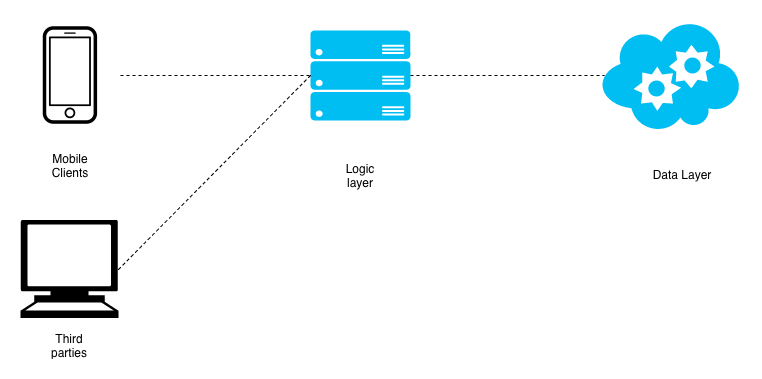
\includegraphics[height=6.00cm,keepaspectratio]{Figures/GeneralSchema}
	\caption{High level view of the system's architecture}
\end{figure}

\begin{figure}[h!]
	\centering
	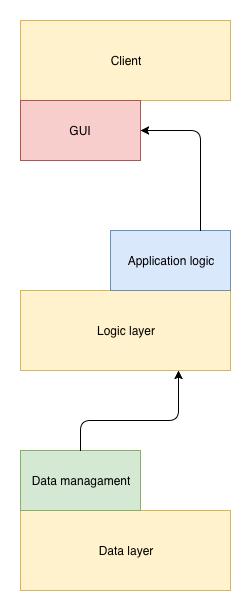
\includegraphics[height=8.00cm,keepaspectratio]{Figures/ThreeTierSchema}
	\caption{Distribution of application's function among the tier}
\end{figure}

The decision of this kind of architecture has been taken in order to build the system in the most modular possibile way. Here are described layer organisation:

\begin{itemize}
	\item Presentation layer:\begin{itemize}
			\item \textit{Mobile clients}: users will be given with a iOS application which will be a view of the entire system.
			\item \textit{Third parties}: third parties will be given with a light web interfaces to register/manage API access and they will be authorised to communicate with the system.
			\end{itemize}
	\item \textit{Logic layer}: logic layer will implement all the logic of the entire system and will handle communications between clients' app and the data layer.
	\item \textit{Data layer}: data layer will be implemented in third party's cloud system and will keep persistent users' data.
\end{itemize}

The idea is to keep as separate as possibile the logic layer from the data layer in order to let the system grow in a modular fashion and let us change cloud data provider as the system's dimension grow with the minimum effort.

\subsection{Component view}
\subsection{Deployment view}
\subsection{Runtime view}
\subsection{Component interfaces}
\subsubsection{API structure}

All the api system will be implemented referring to a single endpoint www.data4help.cloud. Users' applications and third parties will refer to different subdomain:

\begin{itemize}
	\item \textit{www.data4help.cloud/api/users} will be the specific endpoint for the application that serves users.
	\item \textit{www.data4help.cloud/api/thirdparties} will be the specific endpoint for thirdparties.
\end{itemize}


\subsection{Selected architectural styles and patterns}
\subsection{Other design decision}
\end{document}